\section{Evaluation}
\label{sec:evaluation}
% We evaluate \OurSys using different types of traffic to measure its improvement
% to application-level behaviour in the presence of lossy links.

We evaluate \OurSys with microbenchmarks and network simulation to answer these questions:
\begin{itemize}

\item What are the resource requirements for \OurSys with different levels of 
error correction?

\item How much does \OurSys improve application throughput across lossy links?

%\item What benefit can \OurSys have to networks at large?
\end{itemize}

\subsection{Setup}
\begin{figure}
  \centering
  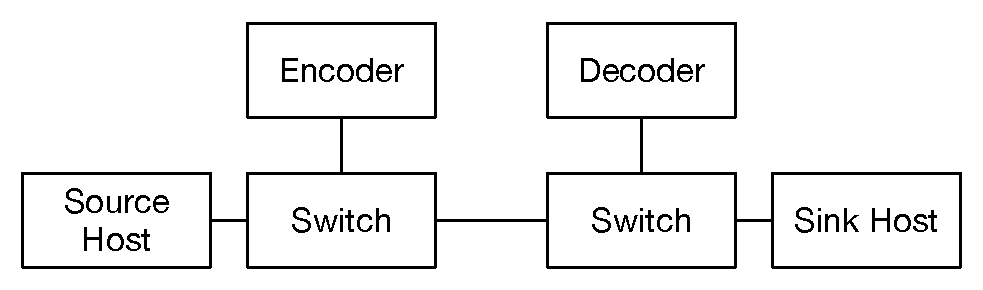
\includegraphics[width=0.3\paperwidth]{exp_topo.pdf}
  \caption{\label{fig:exp_topo} Testbed topology for benchmarks.}
\end{figure}

Figure~\ref{fig:exp_topo} depicts the testbed we used to benchmark \OurSys.
The two traffic generation hosts are each connected to different \OurSys
enabled switches, which are themselves connected by a 10 GbE link. The
switches are Wedge BF32-100X's with Barefoot Tofino~\cite{tofino} P4 
programmable forwarding engines. 

% We
% evaluate three possible deployment models for \OurSys: an FPGA external to
% the switch; a software implementation running on the switch CPU; and an ASIC  
% implementation integrated into the switch forwarding engine. 

\subsection{\OurSys models}

\subsubsection{Line Rate P4 Model.} To measure the effect of faulty links and
\OurSys at the application level, we implemented a P4 program that models
lossy links and the FEC encoder / decoder. The model runs at line rate on the
Barefoot Tofinos in our testbed alongside layer 2 forwarding. It captures
three overheads that are important to applications: the bandwidth overhead
that the encoder adds by inserting parity packets and \OurSys headers; the
latency overhead that the decoder adds when recovering lost packets; and the
transport layer overhead that  drops from corruption add.


\begin{itemize}

\item The \textbf{Encoder Model} encapsulates packets with the \OurSys  header
and generates blank parity packets. It tracks per-port block IDs and  packet
indices using P4 register arrays. It recirculates the largest packet in each
block until the block is complete, then cloning the packet with the Tofino's
multicast engine.

\item The \textbf{Faulty Link Model} adds a header to each packet
indicating whether or not the neighbor switch should consider it lost. It
selects packets for loss according to a simple binomial distribution
implemented with the Tofino's random number generator. The model only 
applies to packets egressing on ports configured to model faulty links. 

\item The \textbf{Decoder Model} applies to all packets ingressing on a
modeled faulty link, before any other forwarding logic. For packets  that are
tagged as not lost, the model removes the \OurSys and loss  headers and allows
them to continue to the standard forwarding  pipeline. Instead of dropping
lost packets, it recirculates them until all the packets  for the block
arrive. The model then decides whether to recover the  lost packets based on
per-block counters for the number of non-lost  data and parity packets. If at
least K data plus parity packets were not lost, the model  "recovers" all of
the lost packets by removing their loss headers and  forwarding them normally.
If recovery fails, the model simply drops the  lost packets without
forwarding.

\end{itemize}

\begin{figure}
  \centering
  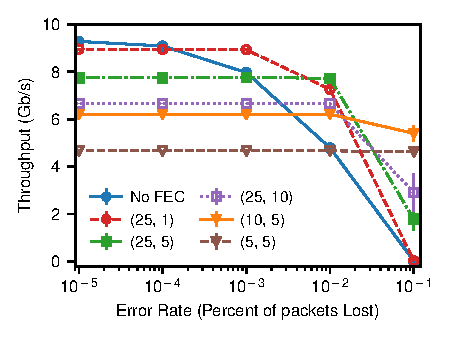
\includegraphics[width=0.3\paperwidth]{figures/lossVsTput.pdf}
  \caption{\label{fig:lossVsTput} Iperf throughput at different loss rates.}
\end{figure}

Figure~\ref{fig:lossVsTput} shows TCP throughput, measured with 60 second Iperf 
trials, as we varied the probability of packet loss. With \OurSys, Iperf sustained 
over 5 Gb/s with loss up to $10^{-1}$ (1 out of every 10 packets dropped). Without 
\OurSys, Iperf's throughput at that level of loss was under 25 Mb/s. 

\OurSys's parity packets reduced throughput at all levels of loss, 
proportional to H. At loss rates greater than or equal to $10^{-4}$ the 
parity packets had less of an impact on TCP throughput than lost packets, for 
most configurations tested. To reduce the overhead of parity packets, the FEC 
can be tuned for the loss rate of each specific link, which is 
stable over time~\cite{corropt}.

Figure~\ref{fig:lossVsLatency} shows UDP latency statistics ...



\subsubsection{Event-based simulation}
Figure/Table~\ref{tab:simulation} shows something about the overall benefit of \OurSys from a network-wide perspective, based on an ns-3 event-driven simulation.
This model has better fidelity than the previous model, but is not run on real hardware. This also means we can simulate larger networks. Here we present data for experiments that are comparable to the setups used in the other evaluations.


\subsection{Encoder Microbenchmarks}
Here we evaluate the implementation directly, not using a model.
Latency and throughput graphs for experiments involving different loss rates, and the encoder working on the CPU and FPGA.
Note: we have not optimised the CPU implementation.


\subsection{FPGA resource consumption}
Table~\ref{tab:microbenchmarks} shows the resource requirements for the FPGA implementations of
\OurSys with different H and K parameters.
%CPU cycles for the software
%implementation are measured using Linux performance counters and averaged over
%X packets,
FPGA requirements are obtained from the Xilinx compiler, and the
timing statistics are measured using ingress and egress timestamps on
the switch.


\begin{table}
% \footnotesize
\begin{center}
\small
% \resizebox{\linewidth}{!}{
\begin{tabular}{ l l l l l } 
\toprule
(H, K) & (5,3) & (10,3) & (20,3) & (40,3) \\
\midrule
\emph{Software} & & & & \\
\cmidrule{1-1}
Cycles & & & & \\
Processing Time (ns) & & & & \\
\midrule
\emph{FPGA} & & & & \\
\cmidrule{1-1}
??? & & & & \\
??? & & & & \\
Processing Time (ns) & & & & \\
\bottomrule

\end{tabular}
% }
\caption{Resource requirements for FPGA and CPU implementations of \OurSys with different configurations.}
\label{tab:microbenchmarks}
\end{center}
\end{table}


%We run \OurSys in 3 configurations: outside the switch, on the switch, and in the switch.
%Time how quickly \OurSys reacts to failing links.
